\section{Stylized facts of financial returns}
\label{section: Data}
In this chapter, the data used to uncover the economic regimes are introduced. The primary index that will be used to estimate the parameters of the HMM is the S\&P 500, however, in order to estimate whether the HMM estimation is persistent across different indices a variety of different indices will be applied in subsequent analysis. The temporal and distributional properties of the additional indices are available in appendix XXX. Initially, decisions related to time horizon and optimal observation frequencies are discussed along with a assessment of which financial data that best captures changing regimes. Once the data of the S\&P 500 index has been introduced and reviewed its distributional and temporal properties are explored in section \ref{subsection: distributional properties} and \ref{subsection: temporal properties}. The objective of the chapter is thus to provide an overview of the data that serves as potential usage for regime detection along with its statistical properties.  

\subsection{Time horizon and frequency of data}
\label{subsection: Data frequency}
When utilising financial market data to uncover economic regime changes, a natural questions arises in terms of which data frequency to use. As described, the objective of DAA is to rebalance the portfolios once a regime shifts has occurred, hence if the regime detection relies on too infrequent data, there is a high probability that several regime shifts will remain hidden. As such, data frequencies longer than a month is not considered. Furthermore, as previously mentioned, macroeconomic data is widely available, however, the data is typically characterised by a data frequency of months or even quarters. Therefore, the data frequency of macroeconomic variables propose a challenge, as historic events has shown that economic regime changes can happen swiftly, evident by the recent COVID-19 recession. As such, monthly data compared to e.g. daily data, greatly increases the risk of slow and insufficient detection of economic regime shifts.
 
Despite of the reasoning just outlined, it should be noted that the use of daily data presents some challenges as well. This is due to the fact that daily returns contain a lot of noise and extreme observations, which are evened out on a monthly basis. Consequently, long-horizon returns tend to be more closely approximated by a Gaussian distribution than returns for shorter time horizons (Campbell et al. 1997). As such, short-term data frequencies complicates the modeling significantly, which can lead to sporadic predictions and less persistence. In addition, the use of daily return frequencies makes the aforementioned link to macroeconomic data more difficult to justify, and therefore it becomes challenging, from a macroeconomic perspective, to argue that economic regime shifts occur since there is no tangible macroeconomic evidence to support this before the data gets collected and released. Despite of the complications associated with short-term data frequencies, the arguments for considering daily as opposed to monthly data frequencies are compelling. 

Furthermore, despite the aforementioned issues with sporadic predictions due to daily data frequencies, Bulla et al. (2011) argued that by relying on daily data it becomes feasible to apply filters that increase confidence whenever a regime change has been detected. As such, research cements the possible of implementing a waiting scheme, in which the portfolio manager would wait several days, when a regime shifts has been detected, before changing the portfolio allocation, thereby minimizing the risk of re-allocating capital based on a wrong signal. In addition, the use of model predictive control (MPC) in section \ref{Subsection: Model predictive control} makes daily data frequencies more justified, since it is not possible to make better return predictions for the assets than their long-term average. As such, looking only a limited number of days into the future is not just an approximation necessary to make the optimization problem computationally feasible, it is also reasonable due to the nature of financial returns.

Bulla et al. (2011) further argued that the use of daily data frequencies increases the amount of data available for markets characterised by a short lifetime, however, many financial indices are old and for these older indices monthly data is more available than daily data. Unsupervised machine learning models, such as HMMs, require large amounts of data to be trained in order to achieve a desired and comfortable level of predictability, and as such, the usage of these heavy data-driven models serve as an argument for relying on monthly data as opposed to daily data. Yet, this thesis favors early detection, due to the reasoning outlined above. As a result, daily data, will be used in the analysis. Lastly, the optimal time horizon used for training the model is debatable, however, it should at least span the time required for a financial cycle to unfold in order to include the performance of DAA strategies in several economic environments. The tuning of this hyperparameter will be subject for further analysis and elaboration in section \ref{Subsection: Model estimation and selection}. Furthermore, it should be acknowledged that, the longer the data horizon the more questionable it becomes whether stationarity of the data-generating process can be assumed (Bulla et al. 2011).

The following sections will include details on the S\&P 500 index used for training the hidden Markov models.
 
\subsection{The S\&P 500}
The S\&P 500 is a stock index comprising 500 companies from the U.S. which was founded in 1957. The stocks that make up the index are selected by a committee which include representation from all major segments in American industry. As such, contrary to prevailing public sentiment, the index is not simply made up of the 500 largest companies in the U.S. The S\&P 500 Index is a market-capitalization weighted index in which the 10 largest companies account for 27.5\% of the capitalization of the index as of per December 2020. Figure \ref{fig: SP500_index} showcases the development of the S\&P 500 Index since origination. 
 
\begin{figure}[H] 
    \centering
    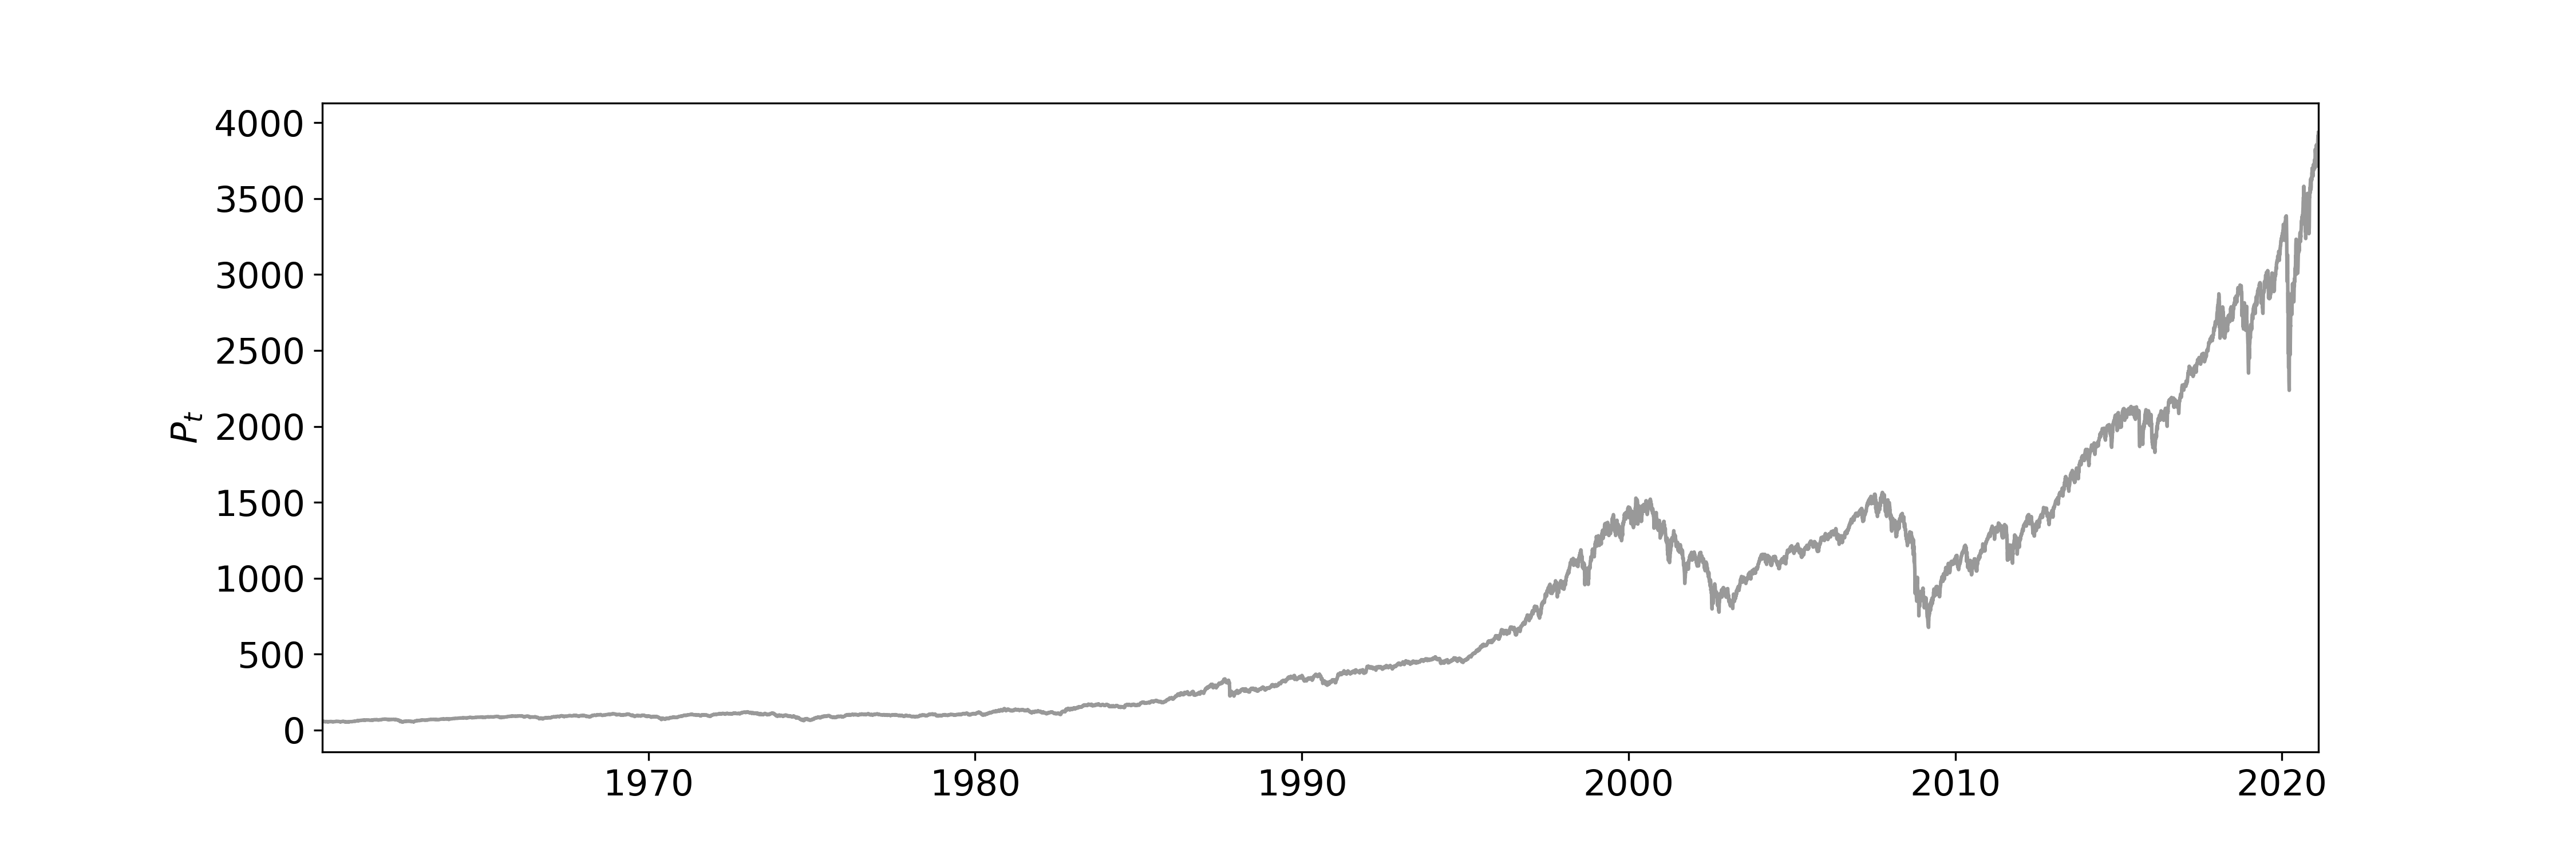
\includegraphics[width=1\textwidth]{analysis/data_description/images/SP500_index.png}
    \caption{Development S\&P 500.}
    \label{fig: SP500_index}
\end{figure}

As is evident from figure \ref{fig: SP500_index} the 44 year data period has been impacted by the major market movements including black monday in October 1987 as well as the dot-com bubble of the late 90s and early 2000s. Furthermore the attractive bull market leading up to the GFC has been well-captured by the development of the S\&P 500 Index. Lastly, the long bull market following the GFC as well as the recent COVID-19 correction and rebound appears to be well-captured by the S\&P 500 Index, thereby indicating that it will serve well for model estimation purposes. Furthermore, another neat property of the S\&P 500 is the fact that it dates back to 1960 hence there is a large amount of data that can be used to train the subsequent HMMs. For comparison popular European indices like the DAX 30 originated in 1999, thus shortening the available data considerably.   

It is unlikely that the recent bullish environment for stocks will continue in perpetuity, since interest rates and inflation, at some point, are likely to start increasing. When that happens, investments towards stocks and indexes can procure short to mid-term monetary losses, however, it is evident from figure \ref{fig: SP500_index} that there appears to be a strong upwards trend historically, thus supporting the argument for capital allocation towards stocks in general.

The inclusion of the S\&P 500 index is based on the fact that it is a one of the leading American indices by market capitalization. In addition, contrary to for instance the Nasdaq Composite Index, the S\&P 500 is not exclusively focusing on a specific sector like information technology, hence it should capture the economics trends across sectors accordingly. As such, the thesis treats it as a baseline index in terms of uncovering economic-regimes. The main critique of using the S\&P 500 index is that it exclusively entail American companies, however, from an economic perspective the U.S. economy serves as a fundamental indicator of how the remaining world economy is progressing, hence it is argued that US stocks will be the first to be impacted by changing economic regime. Taking into consideration the aspect of early regime detection, the fact that the index is composed purely of American companies serves as a strength. Furthermore, North American companies makes up almost 2/3 of alternative indices like the MSCI World, hence no matter which large popular index that will be used will contain a heavy skew and over-representation of American stocks.

\begin{table}[H]
\caption{Summary statistics for the daily S\&P 500 log-returns.}
\centering
\begin{tabular}{c c c c c c c c c} 
\hline\hline
Observations & Mean & STD & Skewness & Excess Kurtosis & Min & Max & First ACF & Annual SR \\
\hline
15,385 & 0.0003 & 0.0103 & -1.0353 & 23.8338 & -0.2290 & 0.1096 & -0.006 & 0.4350 \\
\hline
\end{tabular}
\label{tab:summary_stats_S&P500}
\end{table}
 
It is evident by table \ref{tab:summary_stats_S&P500} that the daily log-returns of the S\&P 500 encompass mean daily returns of 0.0003 combined with a daily standard deviation of 0.0103. Furthermore, the S\&P 500 index is left-skewed, highly leptokurtic and encompass a large range at 0.3386. The surprisingly large range can primarily be attributed to the black monday event of 1987 in which the S\&P 500 was hit particularly hard with a daily return of -22.90\%. These conclusions leads to a Sharpe Ratio of 0.4350, which is somewhat low when compared to optimized portfolio and more diversified indices like the MSCI World (see appendix).

\subsection{Distributional properties} An overview of the development for the S\&P 500 index have been plotted in figure \ref{fig: all_indices_index}, however, the timeline have been adjusted so the most recent 25 years of development have been included. Particularly, the development since the electronification of financial markets is of interest, since many actors, including private investors, gained access to the financial markets due to advancement of technology in the late 90s and early 00s. This means that the first observation is from 04-01-1999 and the last observation is 12-02-2021. 
\begin{figure}[H] 
    \centering
    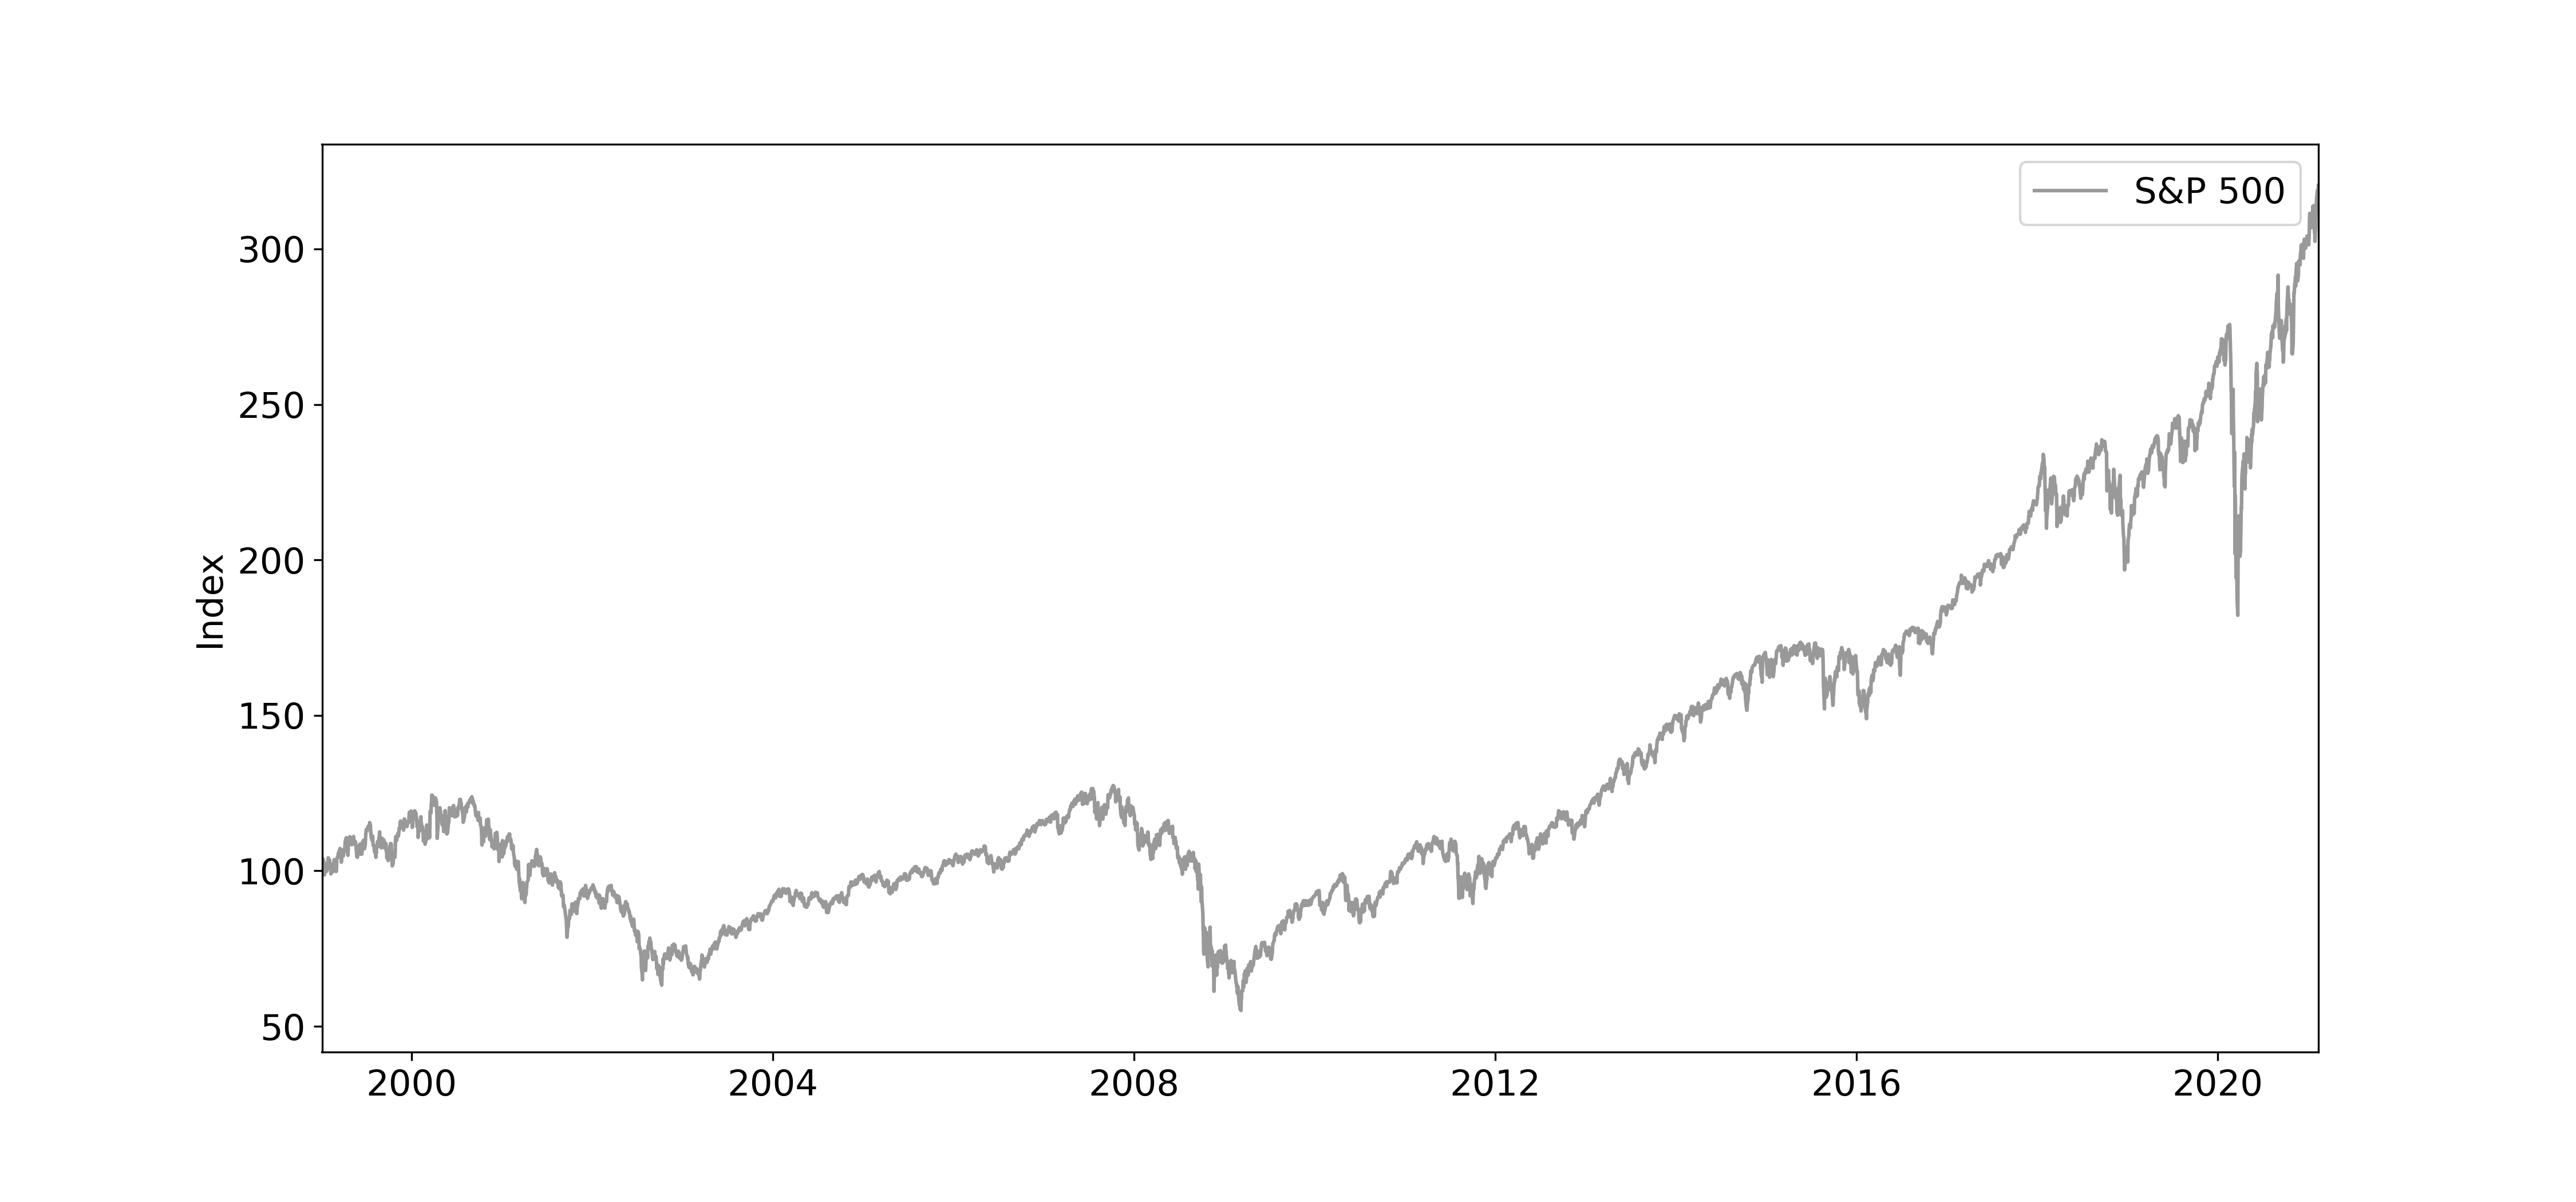
\includegraphics[width=1.0\textwidth]{analysis/data_description/images/adjusted SP500.png}
    \caption{Recent development SP500.}
    \label{fig: all_indices_index} 
\end{figure}

From an overall return perspective it is evident that the S\&P 500 index has been subject to a variety of turbulent market periods including the dot-com bubble and most recently the GFC. Interestingly, the S\&P 500 index only recovered from the dot-com bubble a few months prior to the financial crisis of 2008, yet it was severely impacted by the GFC. In the period following the financial crisis the S\&P 500 has been performing increasingly well resulting in an upward-trajectory until the recent COVID-19 correction, after-which the index reached the present all time high values. 

\subsubsection{Log Returns}
As evident by figure \ref{fig: all_indices_index} the series is not stationary since the mean value is growing and when zooming in on local periods, the development of the index appears to be characterised by strong trends. As such, a transformation is needed to obtain stationary time-series. In cases where the S\&P 500 is characterised by growing means and local trends a log-transformation will narrow the gap between the indices and taking the first difference will eliminate the growing mean values. This results in the log-returns being derived as $r_t = log(P_t) - log(P_{t-1})$, where $P_t$ is the adjusted closing price of the index on day $t$ and $\log$ is the natural logarithm. For daily returns less than 10\%, log returns are a good approximation to the discrete return, as it is the first order Taylor approximation (Nystrup, 2014).

Table \ref{tab:summary_stats_S&P500} showcases the summary statistics for the daily log-returns of the S\&P 500 together with the annual Sharpe ratio and the Jarque-Bera (JB) test statistic. As already noted the distribution is left skewed and strongly leptokurtic, however, this is not a surprising finding given previous studies conducted by Cont (2001) as well as Granger \& Ding (1995b), in which the stylized facts of financial returns were explored substantially. The critical value for the Jarque–Bera test statistic at a 99.9\% significance level is 14.13, in which table \ref{tab:summary_stats_S&P500} clearly highlights that the Jarque–Bera test strongly rejects the normal distribution for all three indices.  

In addition, it is evident from the plot of the kernel density function in figure \ref{fig: Kernel_distributions} that the log return series are characterised by excess kurtosis relative to a Gaussian distribution. As such, there is too much mass centered around the mean and in the tails compared to the Gaussian distribution. The fat left tail implies that using a Gaussian distribution to model returns will underestimate the frequency and magnitude of downside events (Nystrup, 2014). 

\begin{figure}[H] 
    \centering
    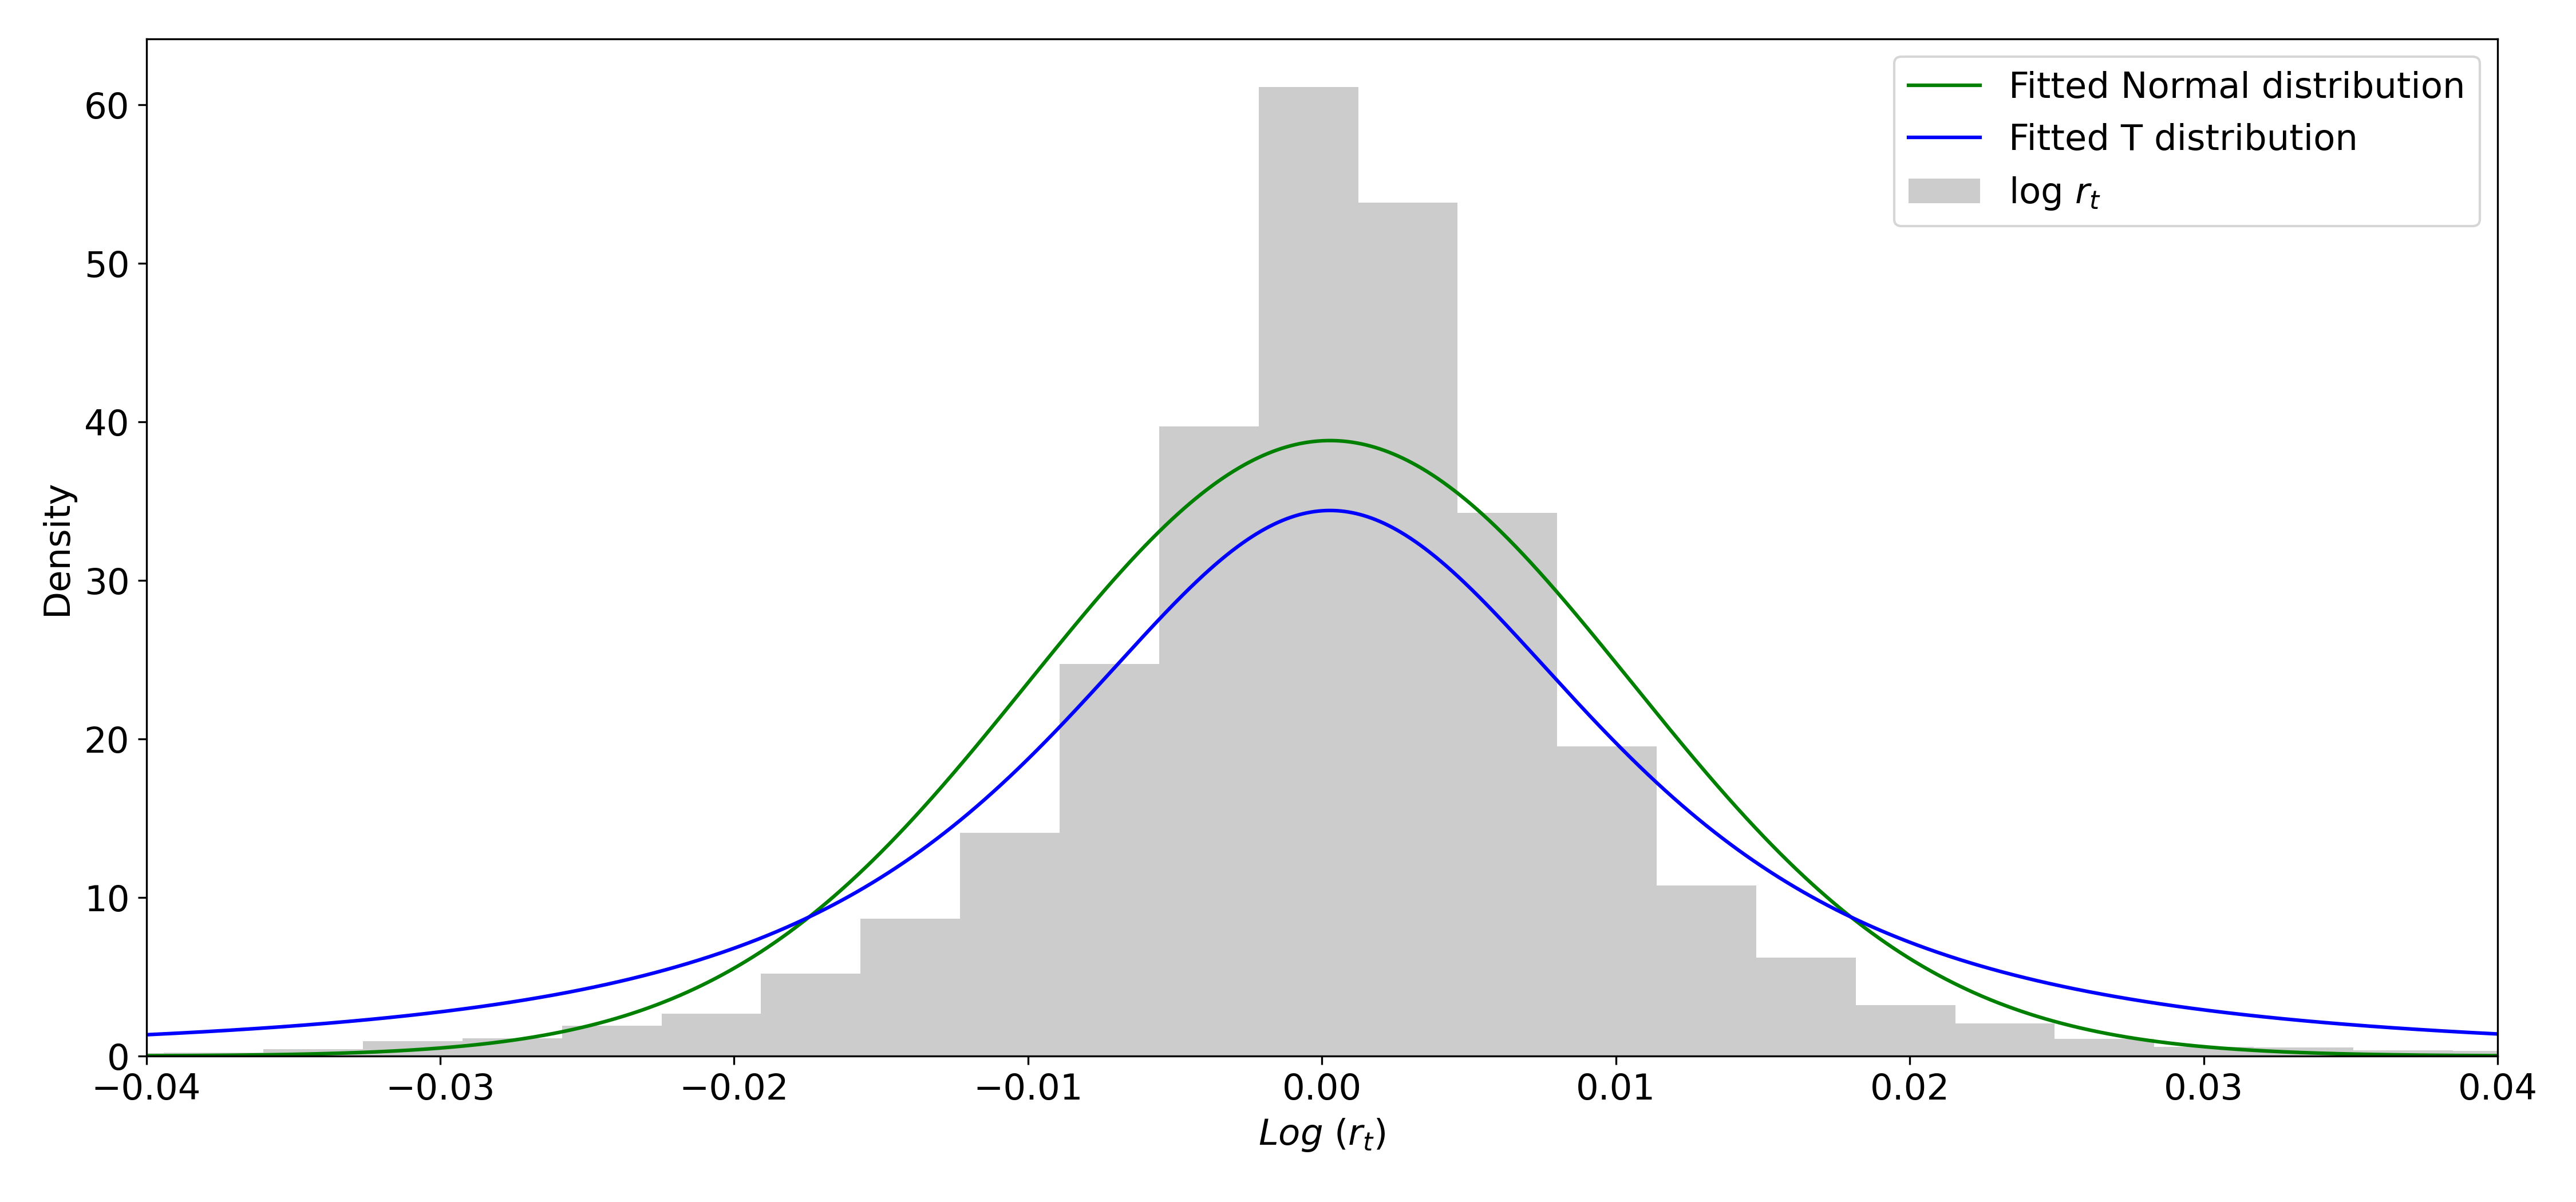
\includegraphics[width=1\textwidth]{analysis/data_description/images/SP500_distribution.png}
    \caption{Distributions. S\&P500.}
    \label{fig: Kernel_distributions}
\end{figure}

Following the properties underlying figure \ref{fig: Kernel_distributions} an interesting analysis would be to uncover how many observations that lie more than 3 standard deviations from the mean. In total there are 219 observations that deviate more than 3 standard deviations from the mean for the S\&P 500 index which is way above the expected 46 if the series followed a Gaussian distribution. Out of these, 108 observations are located in the right side of the tail while the remaining 111 are located in the left tail. This phenomenon that large drawdowns occur more often than similar large upwards movements is well researched and known as the gain/loss asymmetry (Cont, 2001). In addition, it should be noted that since the MSCI World contains 12,941 observations, it only takes a few outliers to reject that the series follow a normal distribution. However, as noted by Cont (2001), financial returns are characterised by a large degree of extreme observations compared to the Gaussian distribution, which is evident by the large excess kurtosis from table \ref{tab:summary_stats_S&P500}.

Lastly, it is important to note the subtle distingshion between outliers and extreme observations since extreme observations deviate considerably from the group mean, yet they may still hold meaningful information hence they should not be disregarded.
Since extreme events happen in live markets the observation that they create should be included in the model estimation in order for the model be as realistic as possible. As such, a plot of the log returns for all the indices have been constructed in figure \ref{fig: log_returns_all_indices}

\begin{figure}[H] 
    \centering
    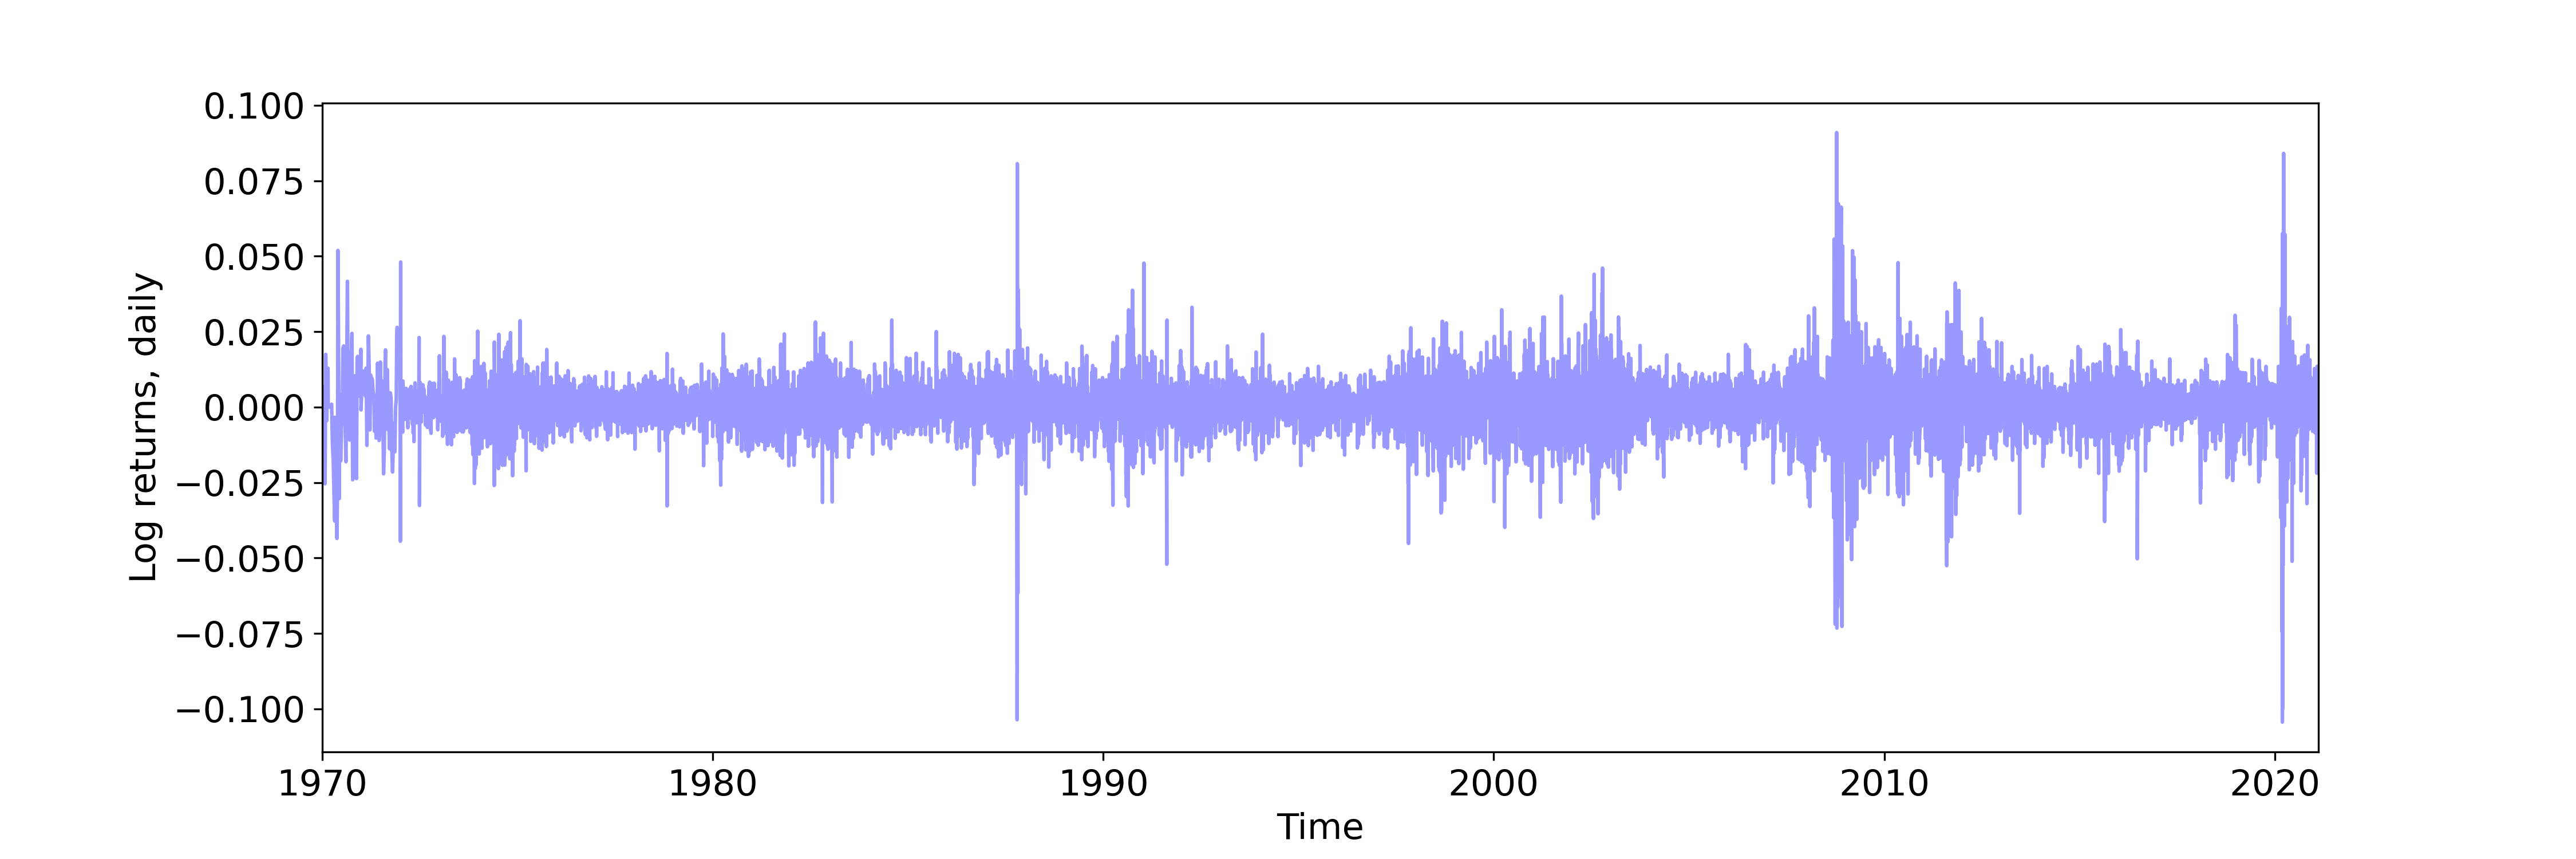
\includegraphics[width=0.65\textwidth]{analysis/data_description/images/MSCI_log_returns.png}
    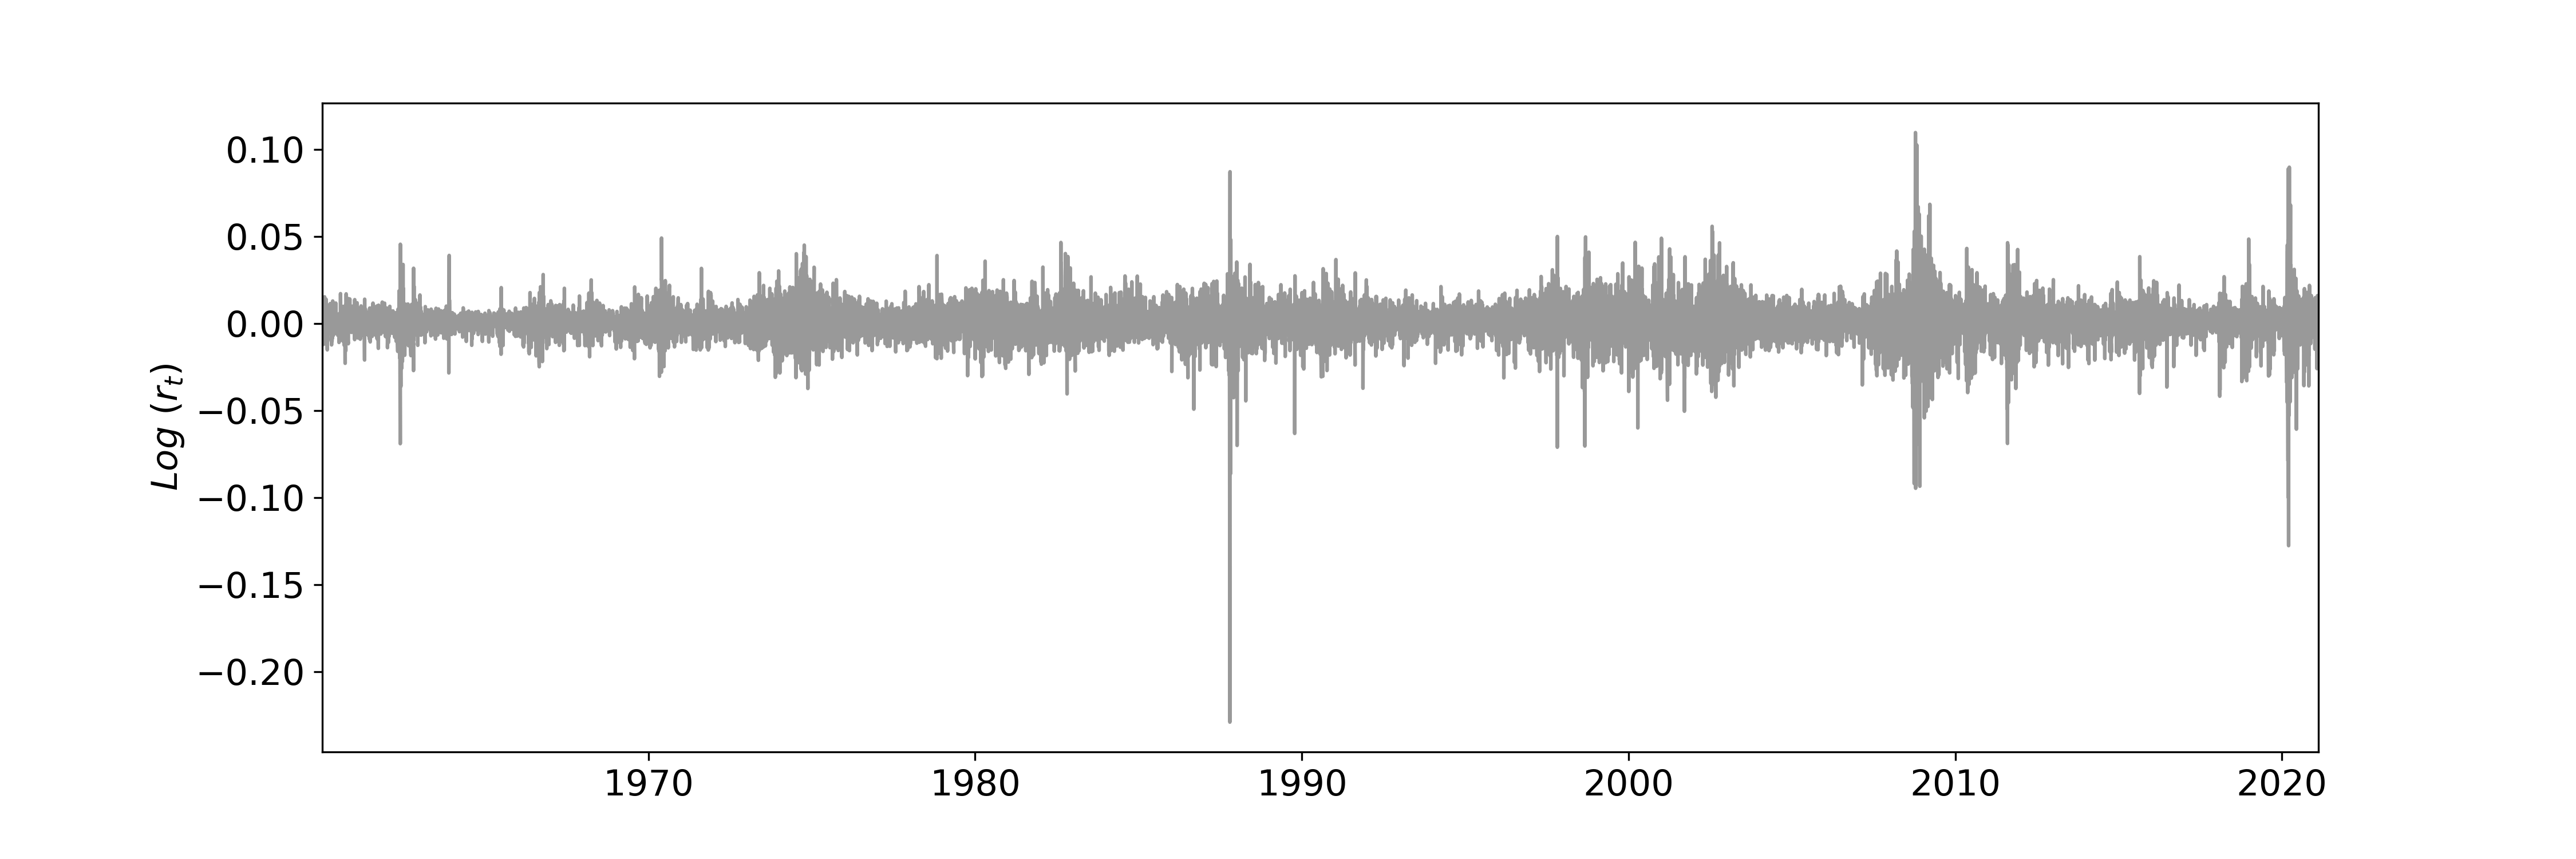
\includegraphics[width=0.65\textwidth]{analysis/data_description/images/SP500_log_returns.png}
    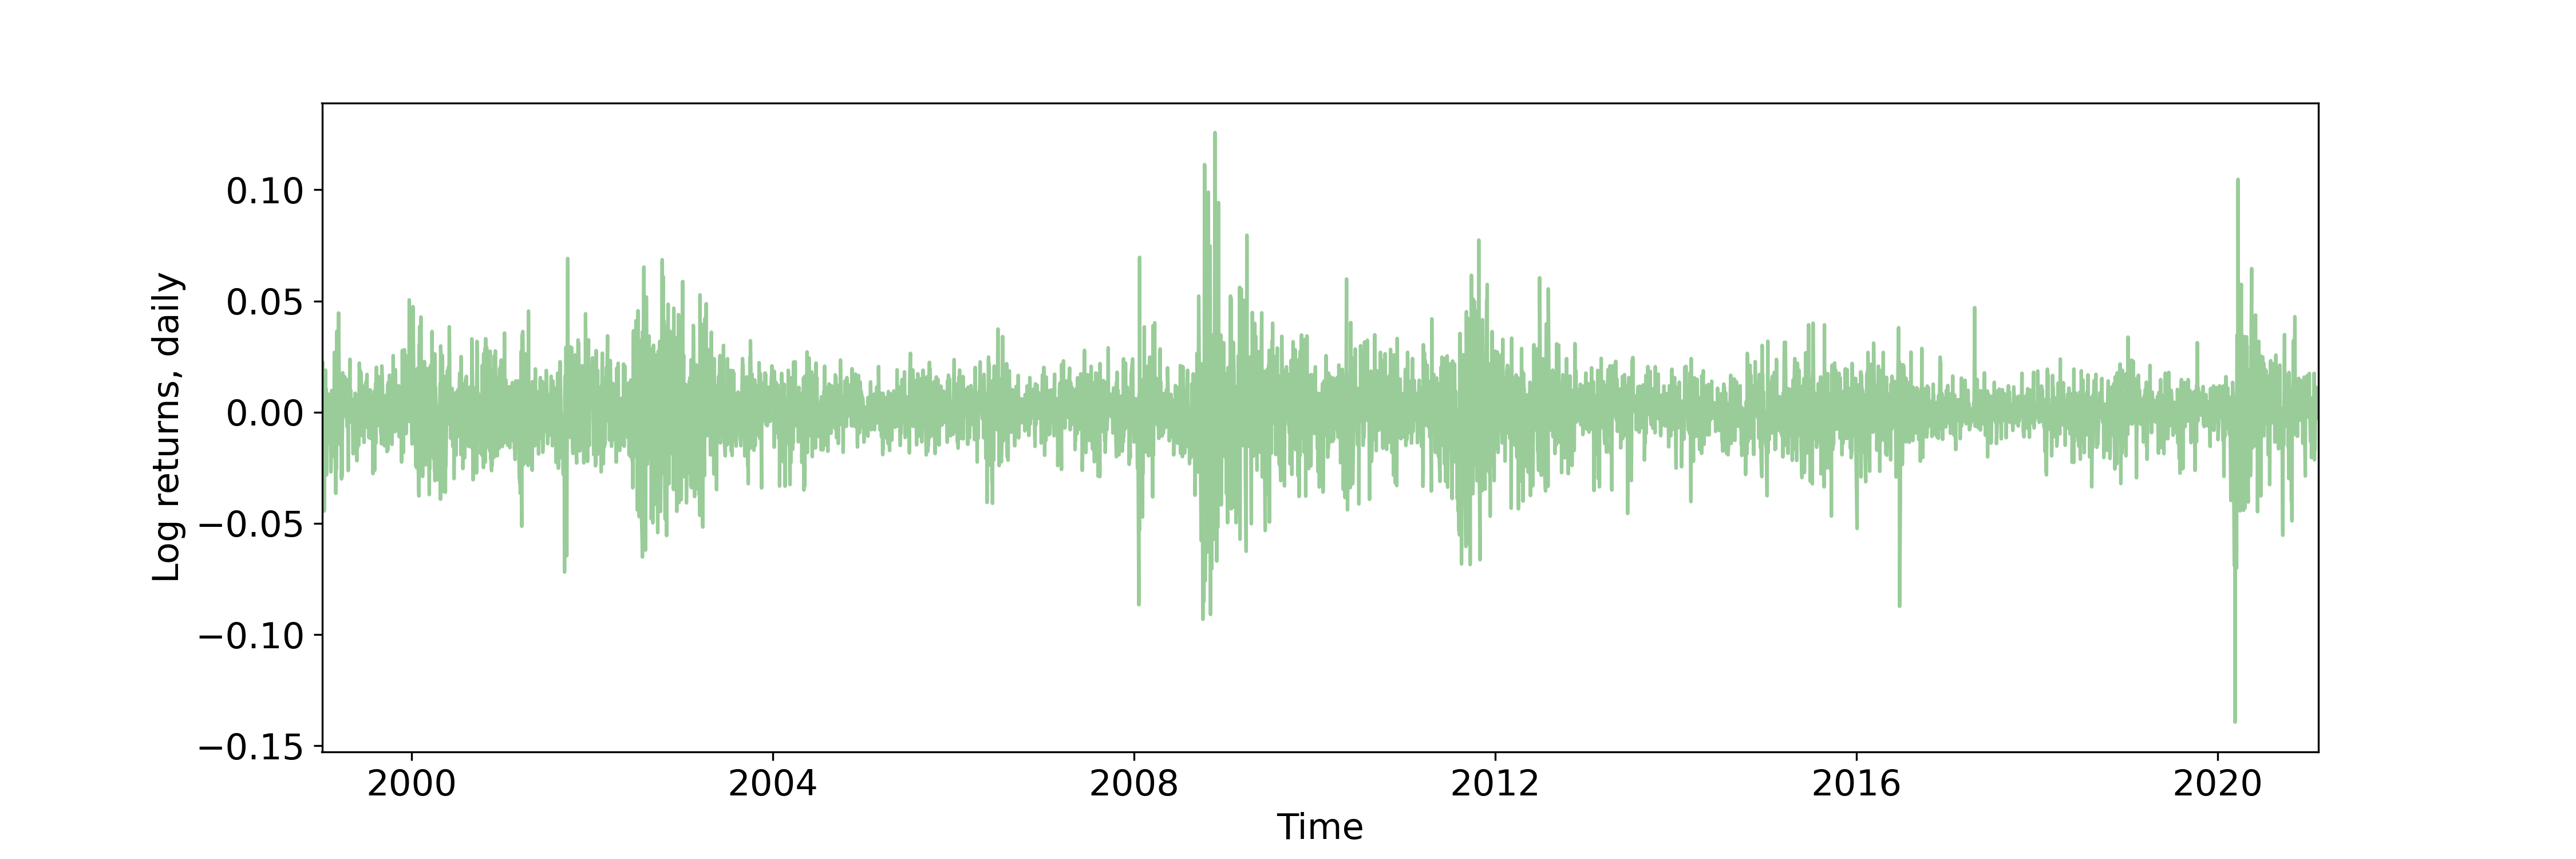
\includegraphics[width=0.65\textwidth]{analysis/data_description/images/DAX_log_returns.png}
    \caption{Log returns. MSCI, S\&P500 and DAX respectively.}
    \label{fig: log_returns_all_indices}
\end{figure}

%%% INDSÆT FIGUR AF LOG RETURNS FOR ALLE INDICES.

\label{subsection: distributional properties}

 
\subsection{Temporal properties}
\label{subsection: temporal properties}
It is evident by the plot of the log returns for the different indices in figure \ref{fig: log_returns_all_indices} that the log returns are characterised as mean stationary, since they fluctuate around a constant mean level close to zero for all three indices. Despite this, the log-returns series for all three indices are seen to be more volatile in some periods. The effect that large prices movements tend to be followed by other large price movements, but not necessarily in the same direction, is known as volatility clustering (Cont, 2001). 

Particularly the MSCI World and S\&P 500 index appear to have increasing volatility throughout time, whereas the DAX 30 appears to have similar or slightly contracting volatility levels. This is not surprising as the MSCI World and S\&P 500 index include observations beginning from the 1970s and 1960s respectively. During these times, there were no active derivative markets and much fewer actors had direct access to trading financial instruments. As such, markets were simpler, less risky and thus characterised by an overall lower level of volatility. 

\begin{figure}[H] 
    \centering
    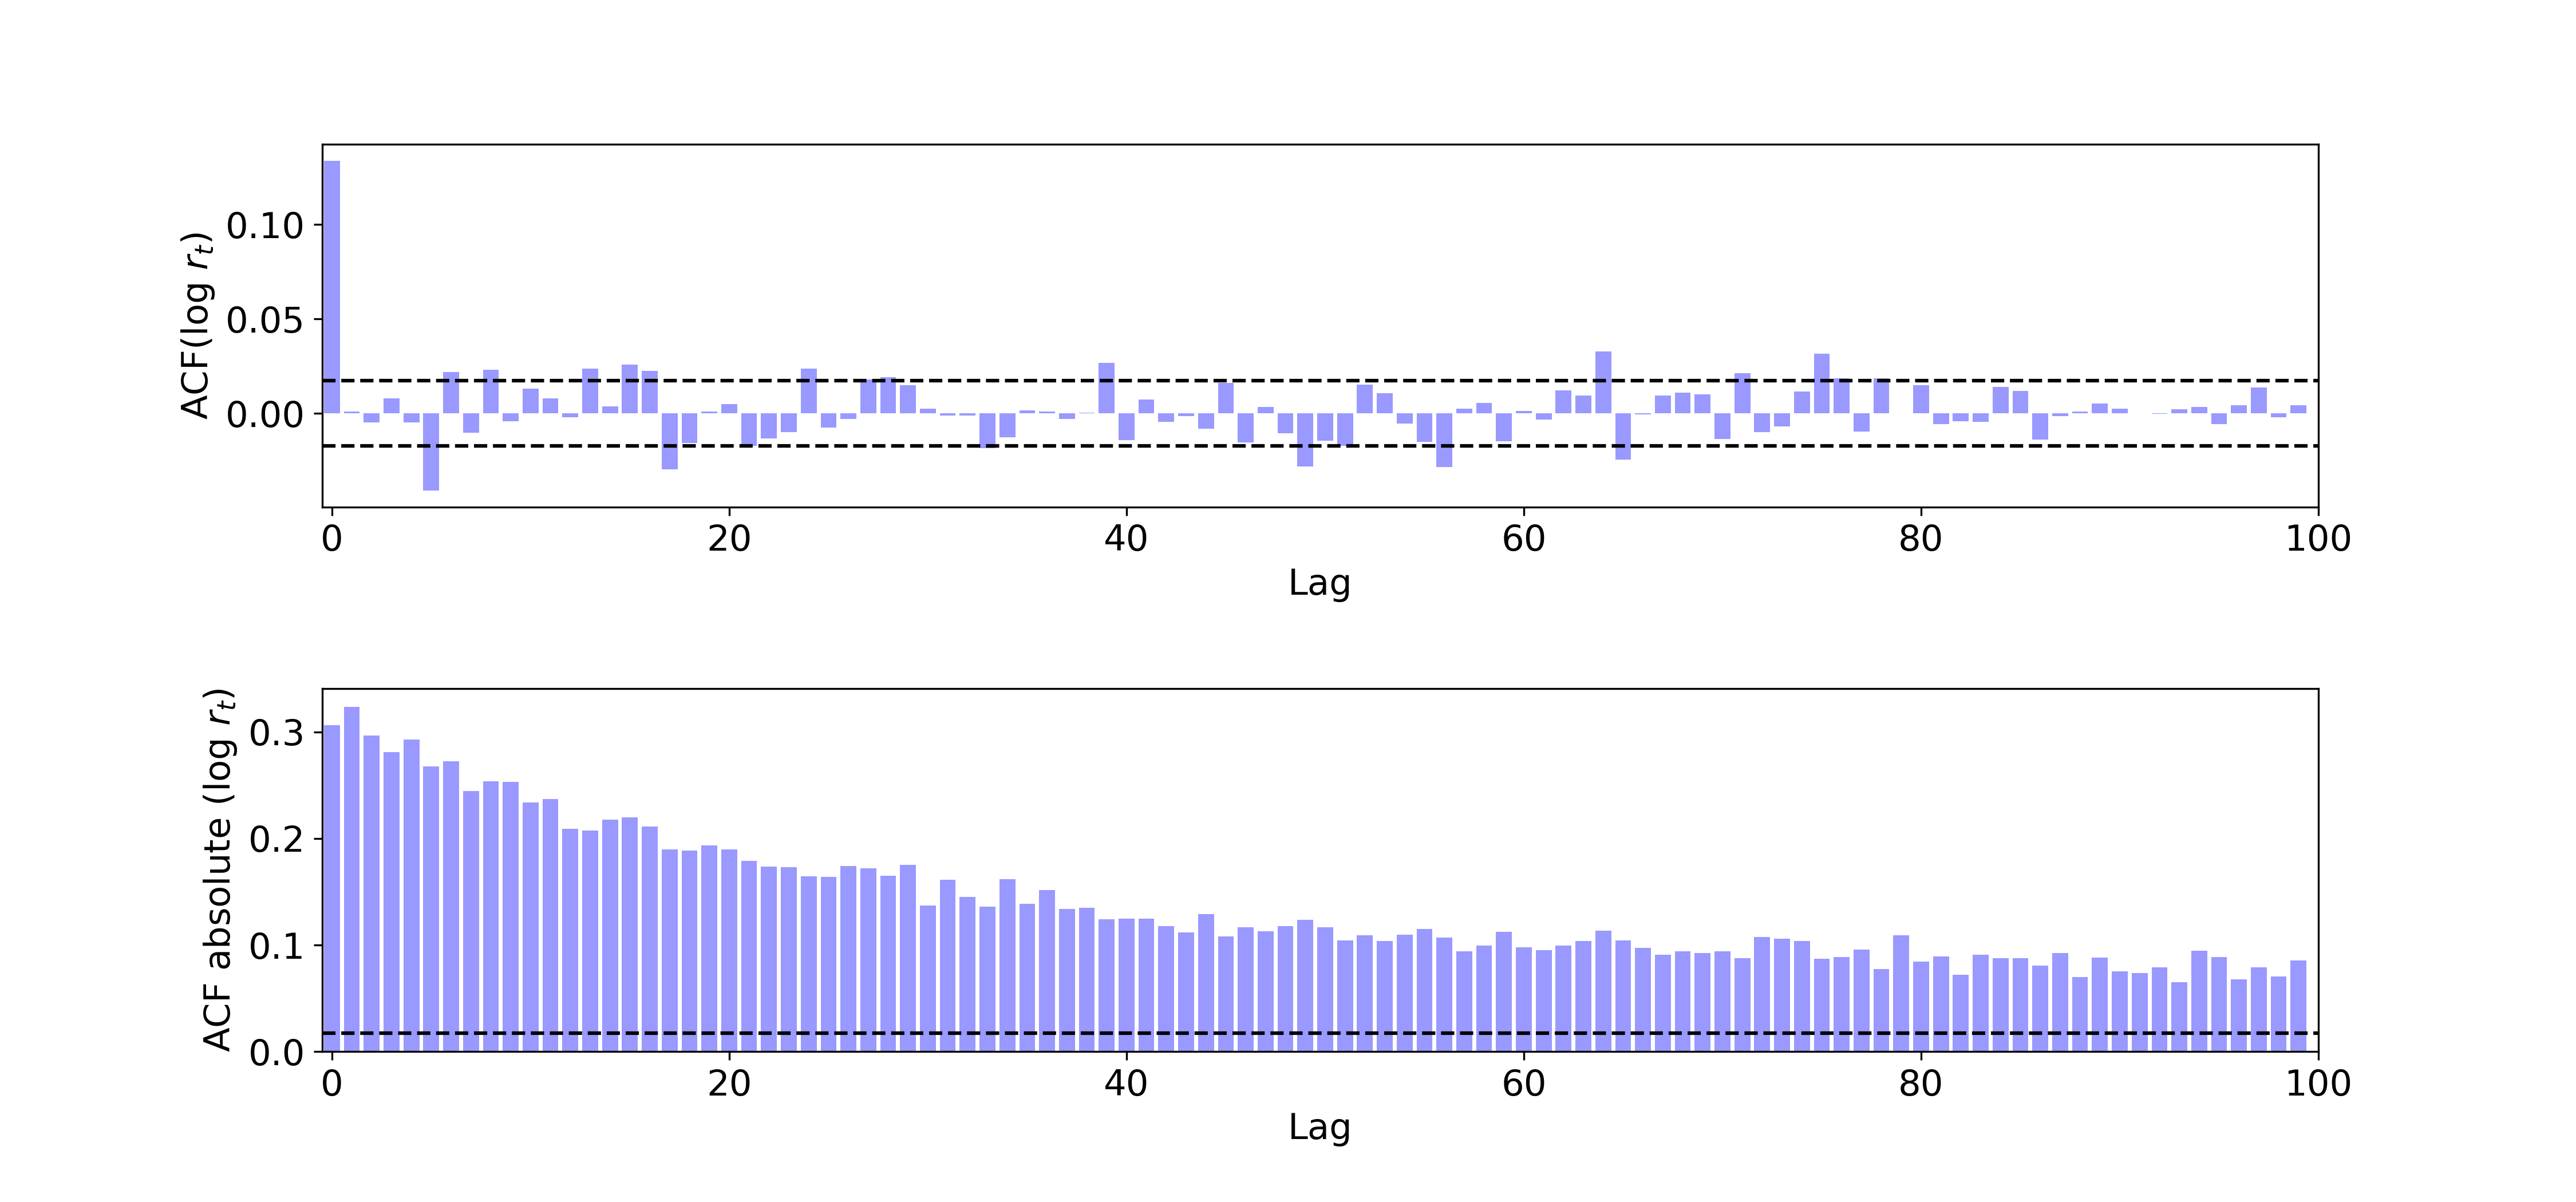
\includegraphics[width=0.65\textwidth]{analysis/data_description/images/MSCI_ACF.png}
    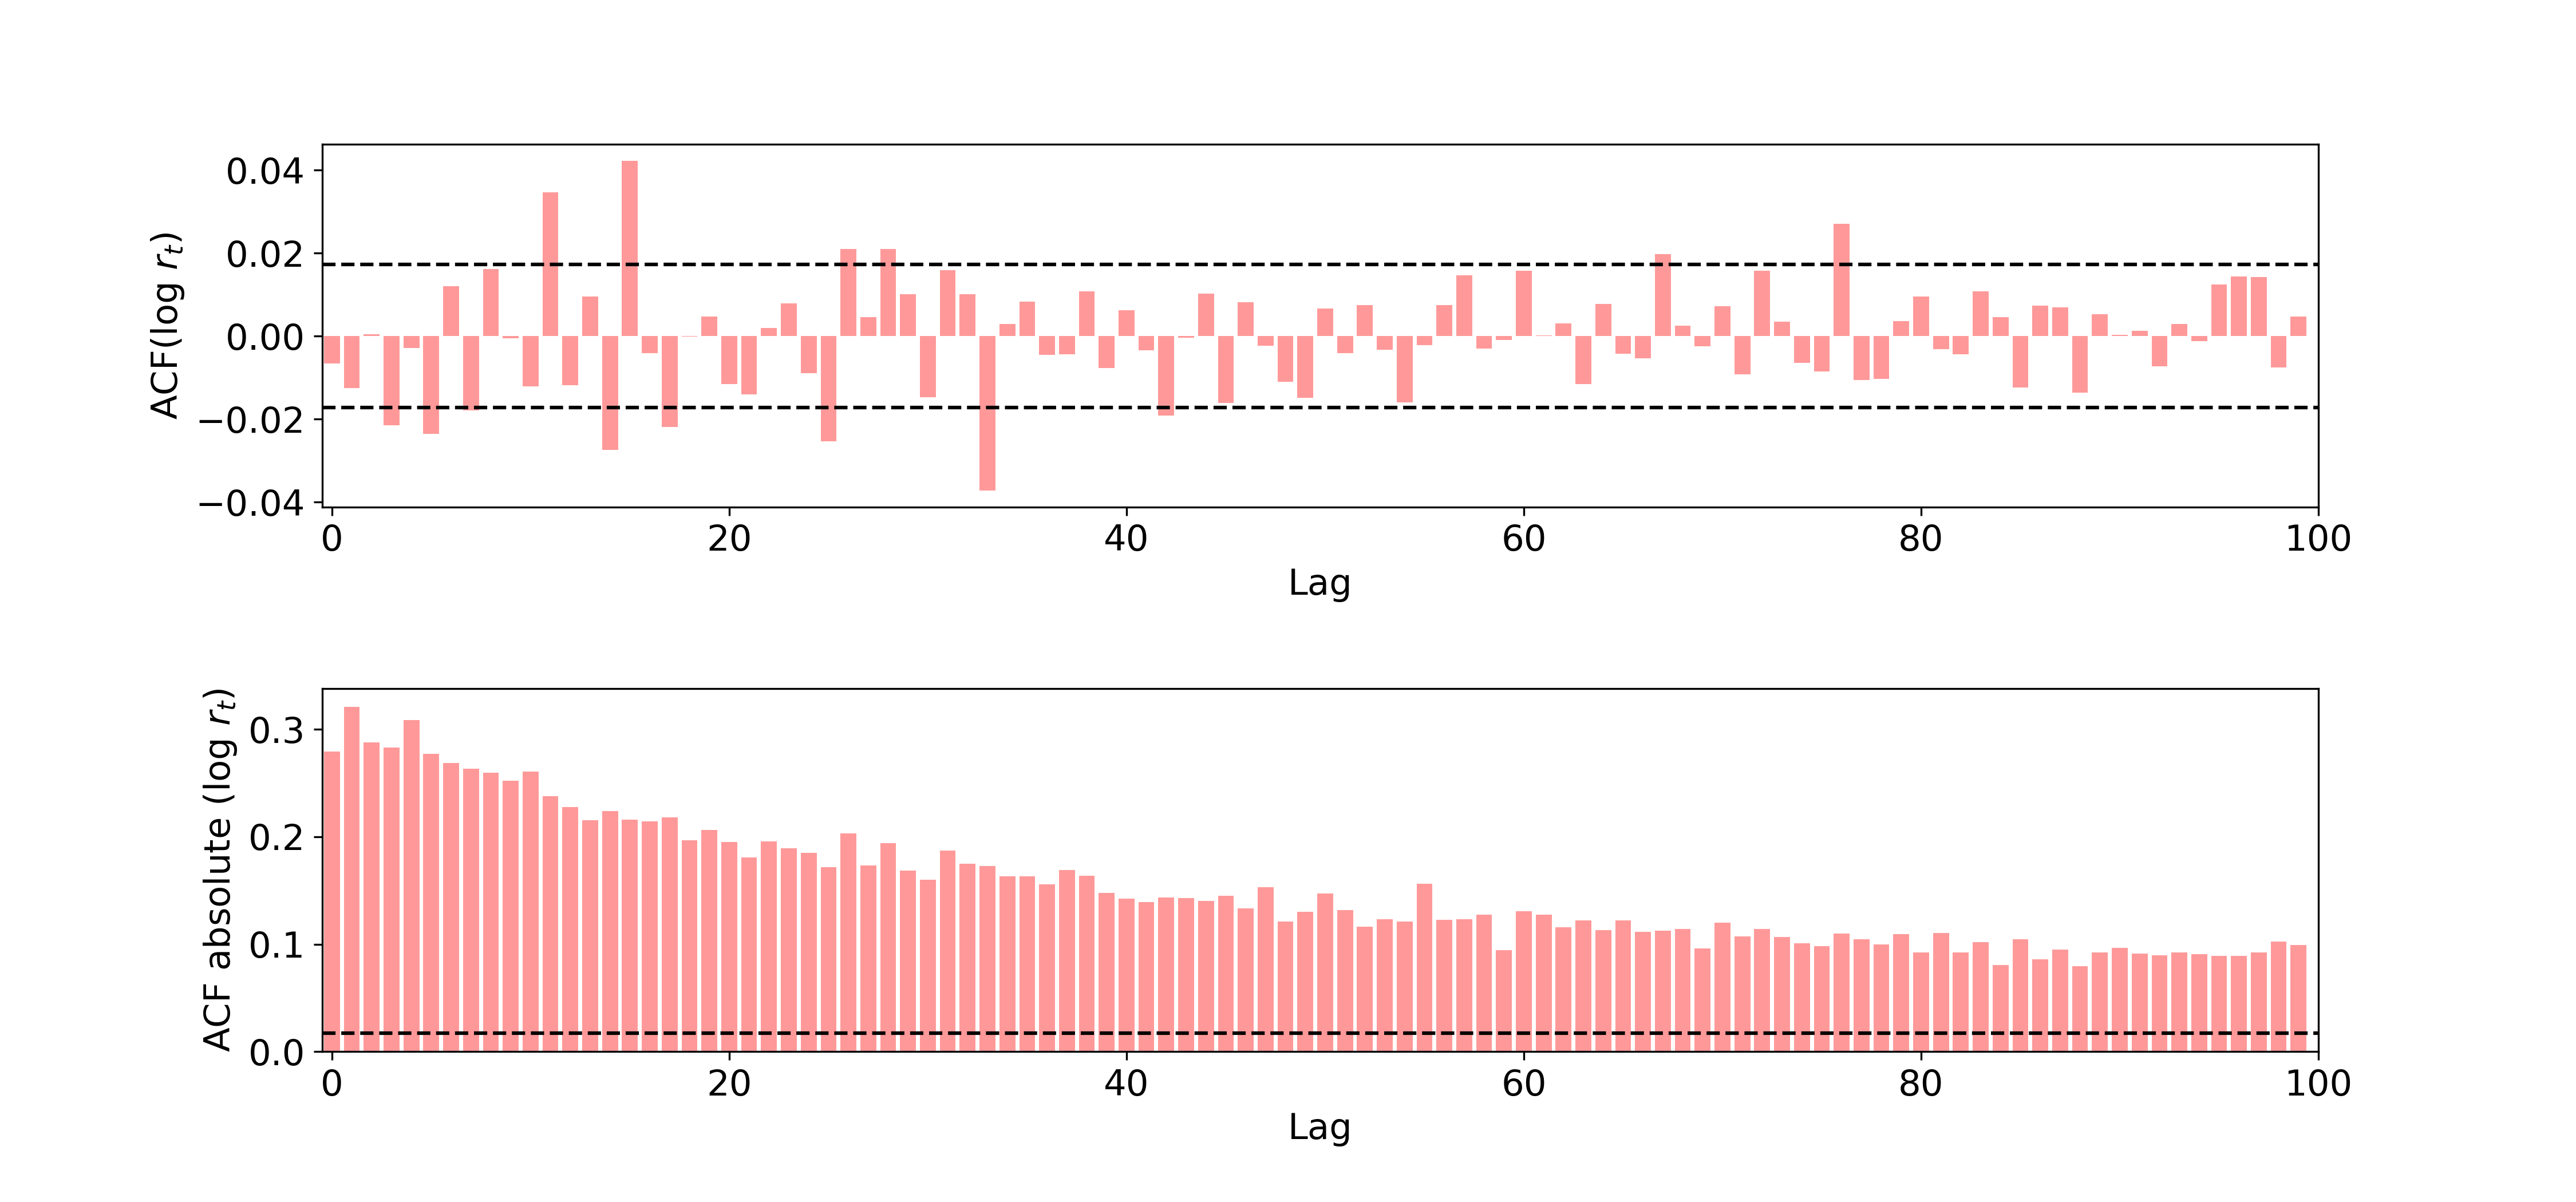
\includegraphics[width=0.65\textwidth]{analysis/data_description/images/SP500_ACF.png}
    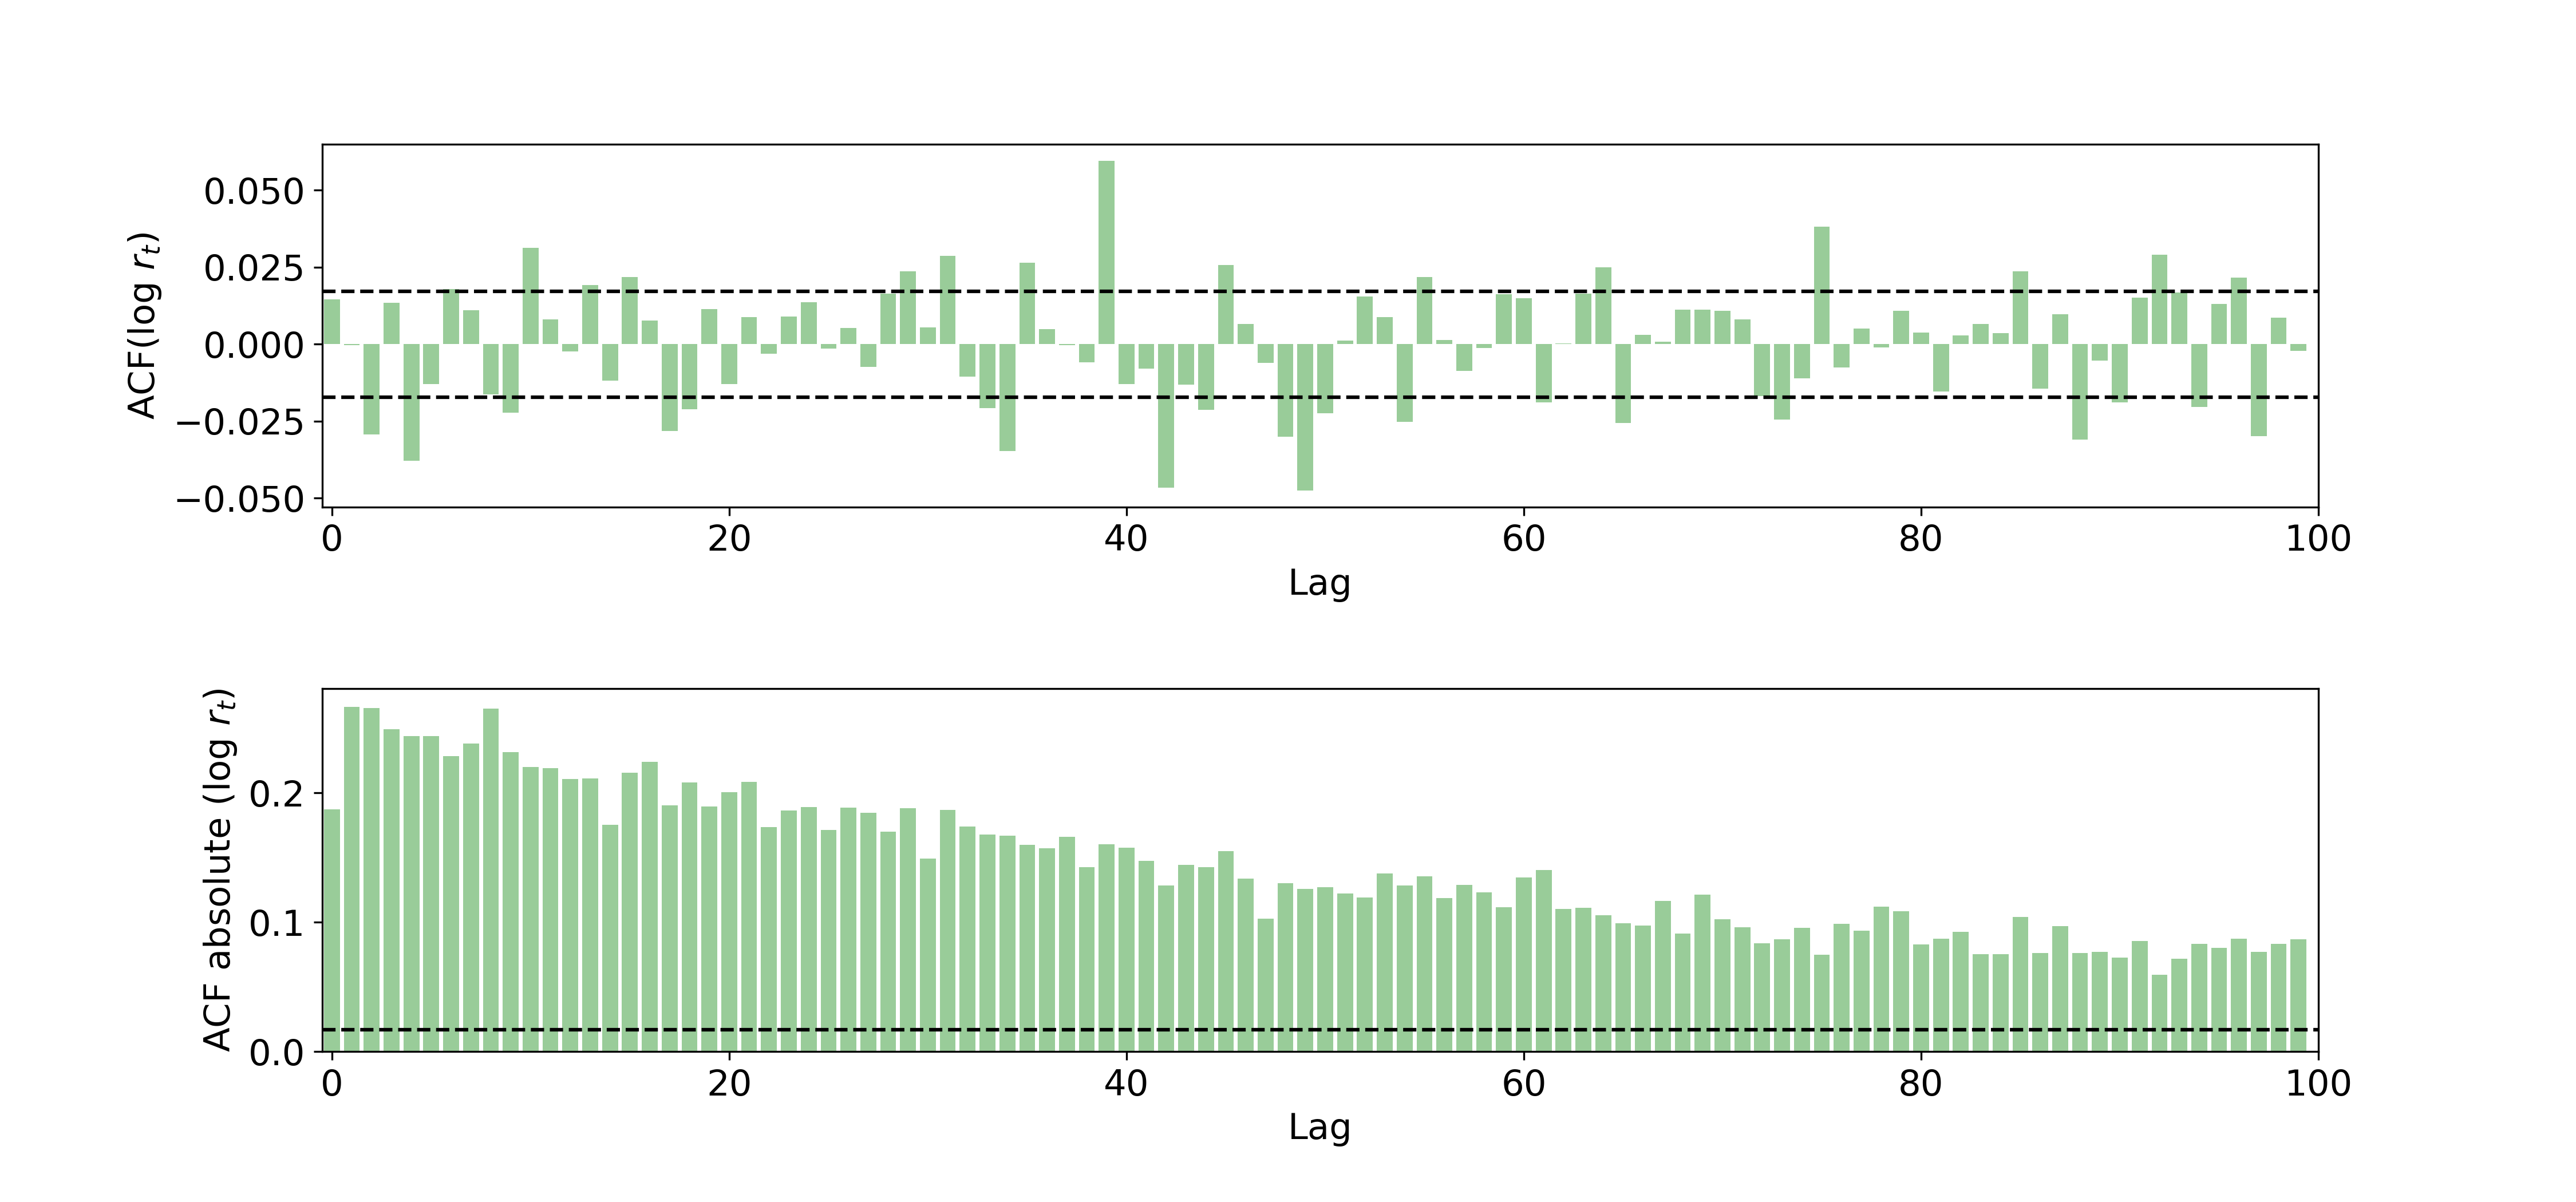
\includegraphics[width=0.65\textwidth]{analysis/data_description/images/DAX_ACF.png}
    \caption{ACF and absolute ACF. MSCI, S\&P500 and DAX respectively. The dashed black line is the 95\% significance level.}
    \label{fig: ACF_all_log_returns}
\end{figure}

The autocorrelation functions (ACFs) for the log-returns and the absolute log returns are shown in figure \ref{fig: ACF_all_log_returns}. The first-order autocorrelation is only significant for the MSCI World index. However, the reader should note that the ACF is time-varying, thus if one were to zoom in on a narrower time-period it is highly probable that the first-order autocorrelation could be significant for all indices. 

The absolute ACFs show significant autocorrelation that persists all the way up to lag 100 for all the selected indices. This suggests that financial returns exhibit a memory component, thereby making volatility somewhat predictable. As such, the long memory of the absolute log-returns is closely related to the previously described volatility clustering from figure \ref{fig: log_returns_all_indices}.

Conclusively, the reader should note that the correlation among the indices are stronger at the times of high market volatility. This is perhaps not surprising since the indices are made up of stocks, however, it highlights that diversification based on investing in different sectors or geographical areas may not materialize precisely when an investor needs it the most. The impact would most probably be less significant if one were to compare a stock index with a bond index, since the correlation would be lower, especially during periods of high volatility. Despite the fact that correlations increased in high volatility markets, there are definitely benefits related to diversification between asset classes.